\section{Governing equations and numerical models}\label{model} 
We consider a self-gravitating, inviscid fluid disc of mass $M_d$ 
orbting a central star of mass $M_*$. We will mainly examine two-dimensional
(2D, or razor-thin) discs in favour of numerical 
resolution, but have also carried out some three-dimensional (3D) disc
simulations. Thus, for generality we describe the system in
3D, using both cylindrical $(R,\phi,z)$ and spherical polar
coordinates $(r,\theta,\phi)$ centred on the star. 
The governing fluid equations in 3D are  
\begin{align}
  &\frac{\p\rho}{\p t} + \nabla\cdot\left(\rho\bm{v}\right) =
  0,\label{cont_eq}\\
  &\frac{\p\bm{v}}{\p t} + \bm{v}\cdot\nabla\bv = -\frac{1}{\rho}\nabla
  p -\nabla \Phi_\mathrm{tot}\label{mom_eq},\\ 
  & \nabla^2\Phi_d = 4 \pi G \rho \label{poisson}, 
\end{align}
where $\rho$ is the mass density, $\bm{v}=(v_r,v_\theta,v_\phi)$ the
fluid velocity, $p$ is the pressure and the total potential
$\Phi_\mathrm{tot} = \Phi_* + \Phi_d$ consists of that from the
central star, 
\begin{align}
  \Phi_*(r) = -\frac{GM_*}{r}, 
\end{align}
where $G$ is the gravitational constant,  and the disc potential
$\Phi_d$. We impose a locally isothermal equation of state 
\begin{align}
  p = c_s^2(R)\rho,
\end{align}
where the sound-speed is given by 
\begin{align}\label{sound-speed}
  % c_s(R) = hR_0\Omega_k(R_0)\left(\frac{R}{R_0}\right)^{-q/2}, 
  c_s(R) = c_{s0}\left(\frac{R}{R_0}\right)^{-q/2}
\end{align}
where $c_{s0} = h R_0\Omega_k(R_0)$ and 
$h$ is the disc aspect-ratio at $R=R_0$, 
$\Omega_k=\sqrt{GM_*/R^3}$ is the midplane Keplerian frequency, and
$q$ is the imposed temperature gradient (since, for an ideal gas the
temperature is proportional to $c_s^2$). The vertical disc scale-height is
defined by $H=c_s/\Omega_k$. Thus, a strictly isothermal disc with
$q=0$ has $H\propto R^{3/2}$, and $q=1$ corresponds to a 
a disc with constant $H/R$. 

For the simulations presented in this paper, the indirect potential
associated with the non-inertial reference frame is purposefully 
neglected to avoid complications arising from the motion of the
central star. For the adopted disc masses $M_d\lesssim 0.1 M_*$, this
effect is not expected to be significant \citep{adams89,shu90}. Indeed,
simulations in the early stages of this project included the indirect
potential, and yield similar results.  

% ang mom cons
% The locally isothermal
% equation of state allows us to apply standard linear density wave
% theory for results interpretation. 
% This allows us to consider
%an isolated disc.   

The 2D disc equations are obtained by replacing $\rho$ with the surface
mass density $\Sigma$, $p$ becomes the vertically-integrated pressure, 
and the 2D fluid
velocity $\bm{v}=(v_R,v_\phi)$ is evaluated at the midplane, as are
the forces from the potential. In the Poisson equation, $\rho$ is
replaced by $\Sigma\delta(z)$, where $\delta(z)$ is the
delta function. 

\subsection{Disc model and initial conditions}
For the initial disc profile we adopt a modified power-law disc with
surface density given by
\begin{align}
  \Sigma(R) = \Sigma_\mathrm{ref} \left(\frac{R}{R_0}\right)^{-s}\times B(R;
  R_{1}, R_{2}, \epsilon, \delta R), 
\end{align}
where $R_0$ is a reference cylindrical radius and $s$ is the power-law
index describing the smooth disc, and $\Sigma_\mathrm{ref}$ is a
surface density scale chosen by specifying $Q_\mathrm{out}$,
the Keplerian Toomre parameter at $R=R_{2}$,
\begin{align}
  Q_\mathrm{out} = \left.\frac{c_s\Omega_k}{\pi G
    \Sigma}\right|_{R=R_{2}}. 
\end{align}
The bump function
$B(R)$ represents a surface density boost between
$R\in[R_{1},R_{2}]$ by a factor $\epsilon^{-1}>1$,
and $\delta R$ is the transition width between the bump and the
smooth disc. We choose 
\begin{align}
  &B(R) = f_1(R)\times f_2(R),\\
  &f_1(R) = \frac{1}{2}\left(1 - \epsilon\right)\left[1 +
    \tanh\left(\frac{R-R_{1}}{\Delta_1}\right)\right]  + \epsilon,\\
  &f_2(R) = \frac{1}{2}\left(1 - \epsilon\right)\left[1 -
    \tanh\left(\frac{R-R_{2}}{\Delta_2}\right)\right]  + \epsilon,
\end{align}
where $\Delta_1 = \delta R \times H(R_{1})$ and similarly for
$R_{2}$. The bump function mimicks mass built-up at some location in 
the disc. 

In 3D, we assume vertical hydrostatic balance
\begin{align}
  0 = \frac{1}{\rho}\frac{\p p}{\p z} + \frac{\p\Phi_*}{\p z} + \frac{\p
    \Phi_d}{\p z},  
\end{align}
which gives the mass density as 
\begin{align}
  \rho = \frac{\Sigma}{\sqrt{2\pi}H}Z(R,z),
\end{align}
where $Z(R,z)$ describes vertical stratification. In practice, we
numerically solve for $Z(R,z)$ by neglecting the radial self-gravity
force compared to vertical self-gravity, which reduces the equations
for vertical hydrostatic equilibrium to ordinary differential
equations. This procedure is described in \cite{lin12b}. 

Our fiducial parameter values are: $s=2$, $R_{1}=R_0$, $R_{2}=2R_0$,
$\epsilon=0.1$, $\delta R=5$, $h=0.05$ and
$Q_\mathrm{out}=2$. An example of the initial surface density and the
Toomre parameter (see\S\ref{wkb}) is shown in
Fig. \ref{initial_surf}. The transition from the self-gravitating and
non-self-gravitating portions of the disc occur smoothly across
$\sim10H$. Initially there is no vertical or radial velocity
($v_R = v_r = v_\theta = 0$). The azimuthal velocity is initialized to
satisfy centrifugal balance with pressure and gravity,
\begin{align}
  \frac{v_\phi^2}{r} = \frac{1}{\rho}\frac{\p p}{\p r} + \frac{\p
    \Phi_\mathrm{tot}}{\p r}
\end{align}
and similarly in 2D. The angular velocity is $\Omega \equiv v_\phi/R$. 


\begin{figure}
  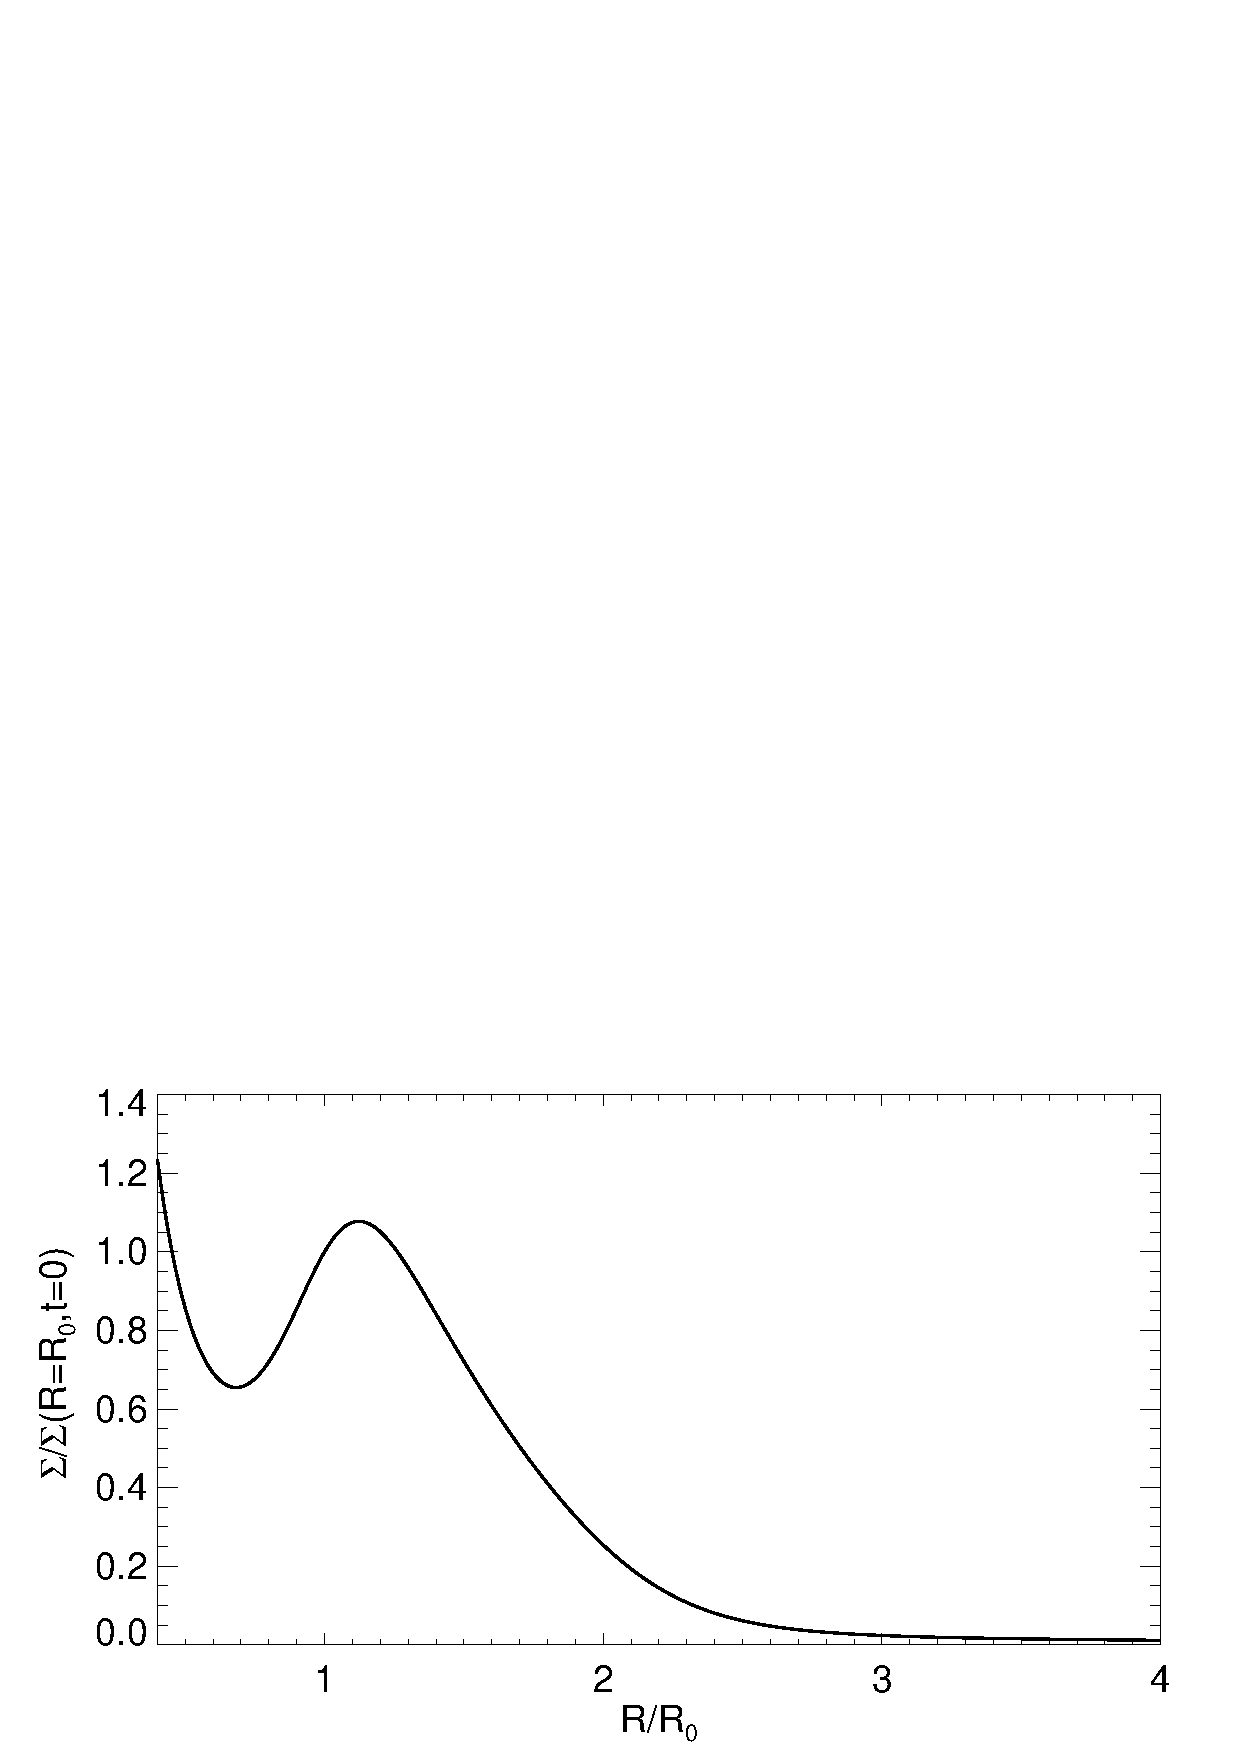
\includegraphics[width=\linewidth,clip=true,trim=0cm 1.7cm 0cm
  0cm]{figures/compare_profiles_dens000} 
  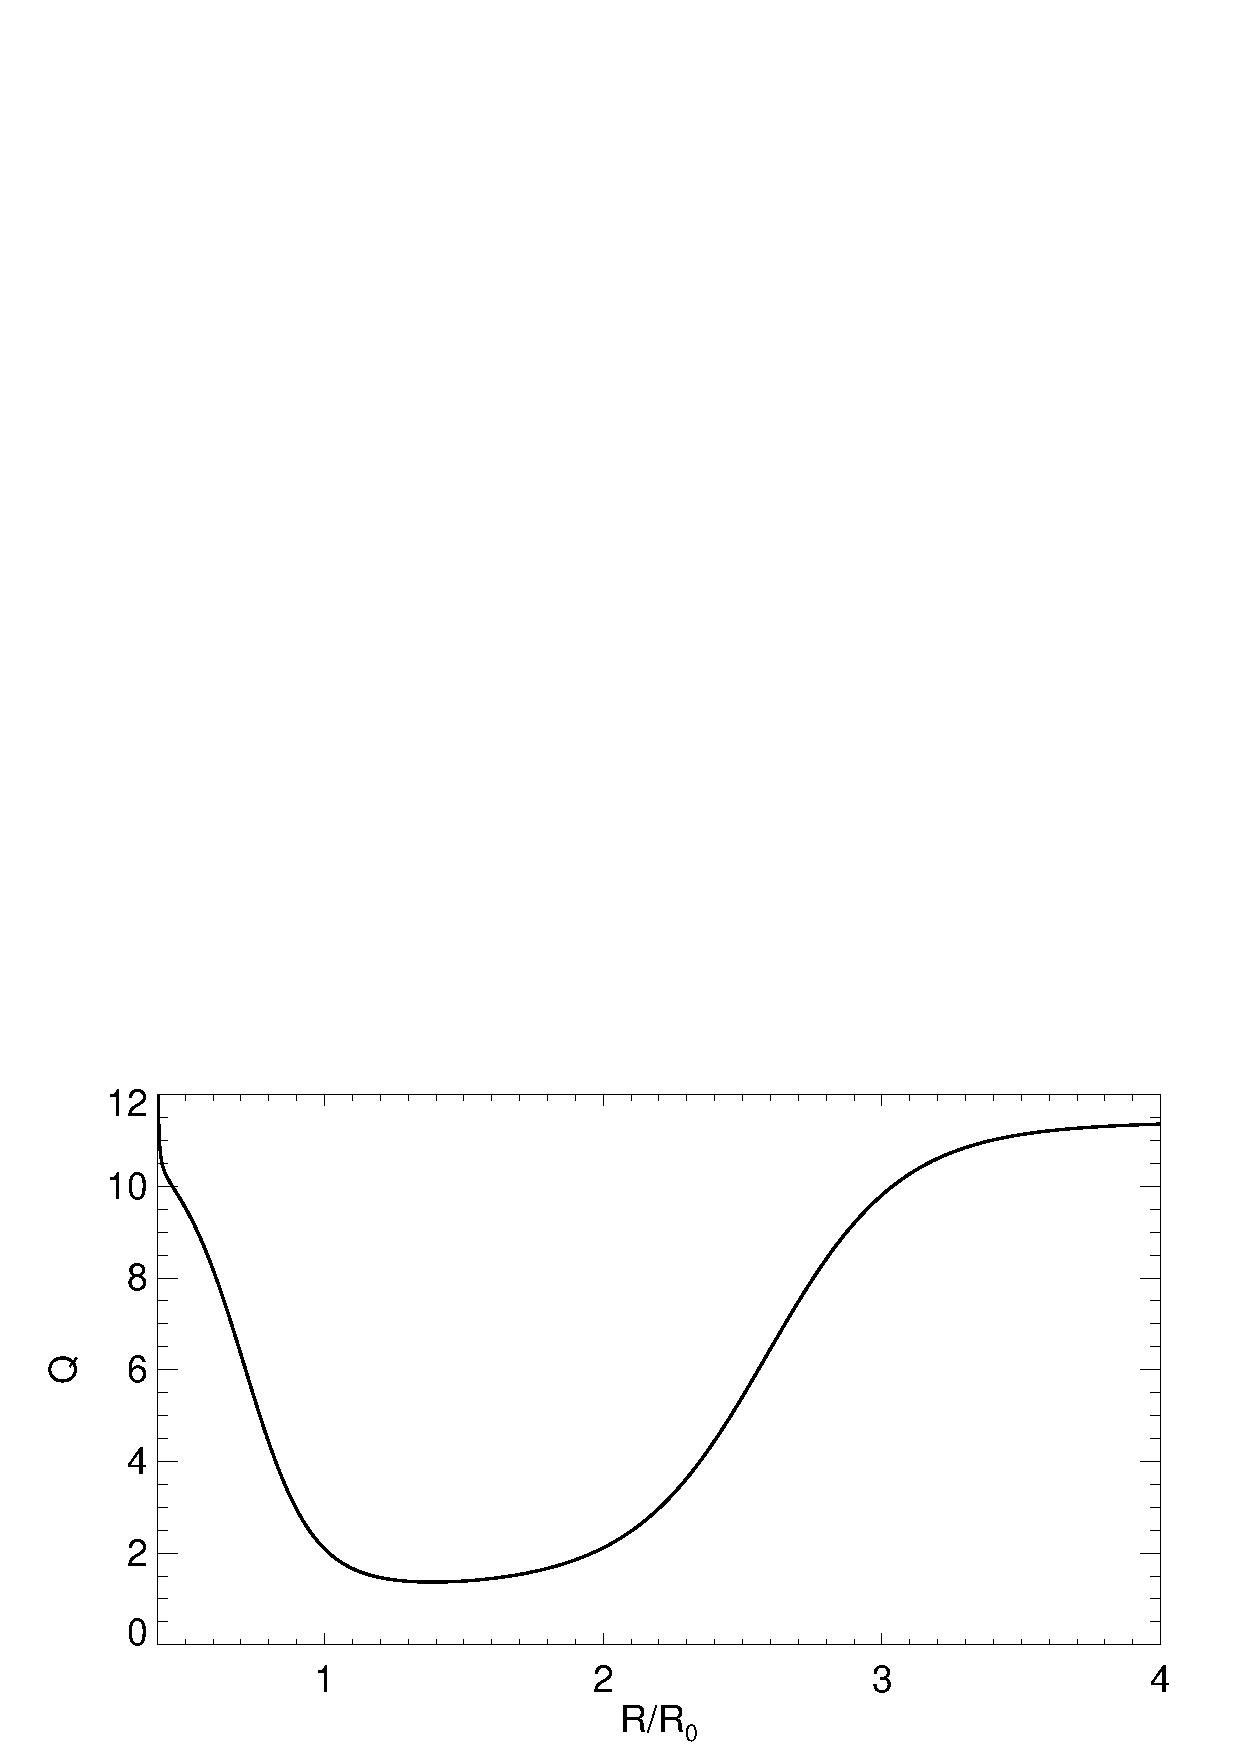
\includegraphics[width=\linewidth]{figures/compare_profiles_Q000}
  \caption{Fiducial profiles of the surface density (top) and Toomre
    parameter (bottom) used in this work.\label{initial_surf}}
\end{figure}

\section{Numerical methods}
We adopt computational units such that $G=M_*=R_0=1$. Time is measured
in the Keplerian orbital period at the reference radius, $P_0\equiv 
2\pi/\Omega_k(R_0)$.  

\subsection{FARGO}
Our primary tool is FARGO with self-gravity \citep{baruteau08}. This
is a popular, simple finite-difference code for 2D discs. `FARGO' refers
to its azimuthal transport algorithm, which circumvents time-step
contraint set by the inner disc boundary \citep{masset00a,masset00b}. 

The 2D disc occupies
$R\in[R_\mathrm{min},R_\mathrm{max}],\,\phi\in[0,2\pi]$ and is 
divided into $(N_R,N_\phi)$ grids, logarithimically spaced in radius and
uniform spaced in azimuth. At radial boundaries we set the
hydrodynamic variables to their initial values.   

The 2D Poisson equation is solved in integral form, 
\begin{align}\label{2d_grav}
  &\Phi_{d,z=0}(R,\phi) \notag \\
  &=-\int_{R_\mathrm{min}}^{R_\mathrm{max}} \int_0^{2\pi}
  \frac{G\Sigma(R^\prime,\phi^\prime)R^\prime dR^\prime d\phi^\prime}{\sqrt{R^2+R^{\prime 2} -
      2RR^\prime\cos{(\phi - \phi^\prime)} + \epsilon_g^2}}, 
\end{align}
using Fast Fouier Transform (FFT), where $\epsilon_g$ is a softening
length to prevent a numerical singularity. The FFT approach requires
$\epsilon_g\propto R$ \citep{baruteau08}. In FARGO, $\epsilon_g$ is
set to a fraction of $hR$.  

% poisson kernal integration, softening 
% where used?
% BC
\subsection{ZEUS-MP}
ZEUS-MP  is a general-purpose finite difference
code \citep{hayes06}. We use the code in 3D spherical geometry, covering
$r\in[r_\mathrm{min},r_\mathrm{max}]$, $\theta\in[\theta_\mathrm{min},\pi/2]$,
$\phi\in[0,2\pi]$. The vertical domain is chosen to cover $n_H$
scale-heights at $R=R_0$, i.e. $\tan{(\pi/2 - \theta_\mathrm{min})}/h=n_H$. 
The grid is logarithmically spaced in radius and uniformly spaced in the angular
coordinates. We assume reflectional symmetry across the midplane, and
apply relfective boundary conditions at radial boundaries and the
upper disc boundary.  

ZEUS-MP solves the 3D Poisson equation using a conjugate gradient
method. To supply boundary conditions to the linear solver, we
expand the boundary potential in spherical harmonics $Y_{lm}$ 
as described in \cite{boss80}. The expansion is truncated at
$(l,m)=(\lmax,\mmax)$. This code was used in \cite{lin12b} for
self-gravitating disc-planet simulations.  

%used in lin 2012 
\subsection{PLUTO} 
PLUTO is a general-purpose Godunov code \citep{mignone07}. The grid
setup is the same as that adopted in ZEUS-MP above. We configure the
code similarly to that used in \cite{lin14}: piecewise linear
reconstruction, a Roe solver and second order Runge-Kutta time
integration. We also enable the FARGO algorithm for azimuthal
transport. 

We solve the 3D Poisson equation throughout the domain using spherical
harmonic expansion \citep{boss80}, as used for the boundary potential
in ZEUS-MP. This version of PLUTO was used in \cite{lin14b} for
self-gravitating disc-planet simulations, producing similar results to
that of ZEUS-MP and FARGO. 

%used in conference proceeding 

\subsection{Diagnostics}

\subsubsection{Evolution of non-axisymmetirc modes}
The disc evolution is quantified using mode amplitudes and angular
momenta as follows. We list the 2D definitions with obvious 3D generalisations. 
A hydrodynamic variable $f$ (e.g. $\Sigma$) is written as 
\begin{align}
  f(R,\phi,t) &= \sum_{m=-\infty}^{\infty}f_m(R,t)\exp{\ii m \phi} \notag\\
  &= f_0(R) + 2 \real\left[\sum_{m=1}^\infty f_m \exp{(\ii
      m\phi)}\right], 
\end{align}
where the $f_m$ may be obtained from Fourier transform in $\phi$. 

The normalised surface density associated with $m$ is
\begin{align}
  \Delta\Sigma_m = \frac{2}{\Sigma_{00}} \real\left[\Sigma_m \exp{(\ii
      m\phi)}\right]
\end{align}
where $\Sigma_{00} = \Sigma_0(t=0)$. The time evolution of the
$m^\mathrm{th}$ mode can be characterized by 
assuming $\Sigma_m\propto\exp{(-\ii \sigma t)}$, where
$\sigma = \omega + \ii\gamma$ is the complex frequency, $\omega$ is
the real frequency and $\gamma$ is the growth rate. The total
non-axisymmetric surface density is 
\begin{align}
  \Delta\Sigma = \frac{\Sigma - \Sigma_0}{\Sigma_0}. 
\end{align}


\subsubsection{Angular momentum decomposition}
The total disc angular momentum is
\begin{align}
  J &= \int_{R_\mathrm{min}}^{R_\mathrm{max}}\int_0^{2\pi} \Sigma Rv_\phi RdRd\phi \notag\\
  &= 2\pi\int_{R_\mathrm{min}}^{R_\mathrm{max}} R\Sigma_0 v_{\phi0} R dR \notag\\ 
  &\phantom{=}+
  \sum_{m=1}^\infty2\pi\int_{R_\mathrm{min}}^{R_\mathrm{max}} 2R\real\left[\Sigma_m v_{\phi
      m}^*\right] RdR 
  %&= \sum_{m=0}^\infty \int _{R_\mathrm{min}}^{R_\mathrm{max}}  j_m(R)
  %dR 
  = \sum_{m=0}^\infty J_m. 
\end{align}
where $^*$ denotes complex conjugation. We shall refer to $J_m$ as the
$m^\mathrm{th}$ component of the total angular momentum, and use it to
monitor angular momentum conservation in the numerical simulations. 
It is important to distinguish this empirical definition from the
angular momentum of linear perturbations, defined through a
conservation law, which is given in \S\ref{wkb}. 

%and we idenfity $J_m$ as the  
%angular momentum associated with disc structure with
%$m^\mathrm{th}$-fold symmetry, and $j_m$ the associated angular
%momentum per unit length. We will use $J_m$ to monitor angular momentum 
%conservation for the disc as a whole.  

\subsubsection{Three-dimensionality}
In 3D simulations we measure the importance of vertical motion with
$\Theta$, where 
\begin{align}\label{theta}
  \Theta^2 \equiv \frac{\avg{v_z^2}}{\avg{v_R^2}+\avg{v_\phi^2}}, 
\end{align}
and $\avg{\cdot}$ denotes the density-weighted average, e.g., 
\begin{align}
  \avg{v_z^2} \equiv\frac{
    \int_{R_1}^{R_2}\int_{\theta_\mathrm{min}}^{\pi/2} \int_{0}^{2\pi}
    \rho v_z^2 dV}{
    \int_{R_1}^{R_2}\int_{\theta_\mathrm{min}}^{\pi/2} \int_{0}^{2\pi}
    \rho dV
  },
\end{align}
and similarly for the horizontal velocities. The radial range of
integration is taken over $r\in[R_1,R_2]$ since this is where
we find the perturbations to be confined. 

\section{Linear density waves}\label{wkb}
In this paper we take a fully numerical approach using non-linear
hydrodynamic simulations. However, it will be useful to employ
existing linear density wave theory to interpret the simulations.
We list here the main definitions and results from 2D linear theory,
taken from \cite{lin11b} and \cite{shu91}.  

In a linear analysis, one assumes a steady axisymmetric background state, such as
that defined in \S\ref{model}, which is then perturbed such that
\begin{align}  
  \Sigma \to \Sigma(R) + \delta\Sigma_m(R)\exp{\left[\ii\left(-\sigma t +
        m\phi\right)\right]}, 
\end{align}
and similarly for other variables. We take $m>0$. Since the background is
axisymmetric, we identify $\delta\Sigma_m(R)\exp{\left(-\ii\sigma
    t\right)} = \Sigma_m$ as defined for diagnostics. 
The linearised mass and momentum equations are
\begin{align}
  &-\ii\sbar \delta\Sigma_m = -\frac{1}{R}\frac{d}{dR}\left(R\Sigma\delta
    v_{Rm}\right) - \frac{\ii m \Sigma}{R}\delta v_{\phi m}, \\
  &-\ii\sbar\delta v_{Rm} - 2\Omega \delta v_{\phi m} = -
  c_s^2(R)\frac{d}{dR}\left(\frac{\delta\Sigma_m}{\Sigma}\right) - \frac{d}{dR}\delta\Phi_m,\\
  & -\ii\sbar\delta v_{\phi m} + \frac{\kappa^2}{2\Omega}\delta v_{Rm} =
  -\frac{\ii m }{R}\left(c_s^2\frac{\delta\Sigma_m}{\Sigma} + \delta\Phi_m\right),
\end{align}
where $\sbar = \sigma - m\Omega$ and $\kappa^2 =
R^{-3}\p_R(R^4\Omega^2)$ is the square of the epicycle frequency. A
locally isothermal equation of state has been assumed.    
The linearised Poisson equation is 
\begin{align}
  \nabla^2\delta\Phi_m = 4\pi G \delta\Sigma_m \delta(z). 
\end{align}

The linearised equations can be combined into a single
integro-differential equation eigenvalue problem. We defer a full
exploration of the linear problem to a future study. Here, we list some
general  properties of the linear perturbations that will be useful
for describing simulation results. 

\subsection{Global angular momentum conservation for linear
  perturbations} 
It can be shown that linear perturbations with $\phi$-dependence in the form
$\exp{(\ii m\phi)}$ satisfies angular momentum conservation
in the form 
\begin{align} 
  \frac{\p \jlin}{\p t} + \nabla\cdot\bm{F} = \tbg, 
\end{align}
\citep[e.g.][]{narayan87,ryu92,lin93b} where
\begin{align}\label{lin_ang_mom_cons}
  \jlin \equiv
  -\frac{m\Sigma}{2}\imag\left(\bm{\xi}^*\cdot\frac{\p\bm{\xi}}{\p
      t} + \Omega \hat{\bm{k}}\cdot\bm{\xi}\times\bm{\xi}^* + \ii
    m \Omega |\bm{\xi}|^2\right) 
\end{align}
is the angular momentum density, $\bm{\xi}$ is the Lagragian
displacement, and $\bm{F}$ is the angular momentum flux
consisting of a Reynolds stress and a gravitational stress. Explicit
expressions for $\bm{\xi}$ can be found in, e.g. \cite{papaloizou85},
and $\bm{F}$ can be read off Eq. \ref{angflux1}.  
% \cite{papaloizou85} and \cite{lin11} respectively, and

% lin papaloizou kley 1993, ryu/goodman, narayan 

The background torque density $\tbg$ is 
\begin{align}\label{baroclinic_torque}
  \tbg \equiv
  -\frac{m}{2}\imag\left(\Sigma_m\xi_R^*\frac{dc_s^2}{dR}\right), 
\end{align}
and arises because we have adopted a locally isothermal equation of
state. In a barotropic fluid, such as a strictly isothermal disc,
$\tbg$ vanishes and the angular momentum associated with
the perturbation is conserved, provided that there is no net angular
momeumtum flux. 

However, as noted in \cite{lin11b}, if there is an imposed
temperature gradient, as in the disc models we consider,
then $\tbg\neq 0$ in general, which corresponds to a torque
exerted by the background disc on the perturbation. We 
outline the derivation of $T_\mathrm{BG}$ in Appendix 
\ref{tbg_deriv}. 

\subsection{Local results}
In the local approximation, perturbations are assumed to vary rapidly
relative to any background gradients. \cite{shu91} gives the
dispersion relation for tightly-wound density 
waves of the form $\exp{[\ii(-\sigma t + m \phi + kR)]}$ in a razor-thin
disc as  
\begin{align}\label{dispersion}
  (\sigma - m\Omega)^2 = \kappa^2 + k^2c_s^2 - 2\pi G \Sigma |k|, 
\end{align}
and $k$ is a real wavenumber such that $|kR|\gg1$. Note that in this
approximation, only axisymmetric perturbations with $m=0$ can be
unstable (having an imaginary $\sigma$).  

Considering a neutral mode, given the real frequency $\omega$ or
pattern speed $\Omega_p\equiv 
\omega/m$, Eq. \ref{dispersion} can be solved 
for $|k|$, 
\begin{align}\label{wavenumber}
  |k| = \frac{\pi G \Sigma}{c_s^2}\left[1 \pm \sqrt{1 -
      Q^2(1-\nu^2)}\right], 
\end{align}
where 
% \begin{align}
%   k_T \equiv \frac{\kappa^2}{2\pi G \Sigma}
% \end{align}
% is a characteristic wavenumber, 
\begin{align}
  Q \equiv \frac{c_s\kappa}{\pi G \Sigma}
\end{align}
is the usual Toomre parameter, and
\begin{align}
  \nu \equiv \frac{(\omega - m\Omega)}{\kappa}
\end{align}
is a dimensionless frequency. In
Eq. \ref{wavenumber}, the upper (lower) sign correspond to short
(long) waves, and $k>0$ ($k<0$) correspond to trailing (leading)
spirals.    

The \emph{co-rotation radius} $R_c$ is where the pattern speed matches
the fluid rotation,
\begin{align}
  \Omega(R_c) = \Omega_p.
\end{align}
\emph{Lindblad resonances} $R_L$ occurs where
\begin{align}
  \nu^2(R_L) = 1. 
\end{align}
Finally, \emph{Q-barriers} occur at radii $R_{Qb}$ where
\begin{align}
  Q^2(R_{Qb})\left[1-\nu^2(R_{Qb})\right] = 1.  
\end{align}
According to Eq. \ref{wavenumber}, purely wave-like solutions with
real $k$ are only possible where $Q^2(1-\nu^2)\leq1$.  

A detailed discussion of the properties of density waves in the local
approximation can be found in \cite{shu91}. An important result is that
waves interior to co-rotation ($R<R_c$) have negative angular momentum, while
waves outside co-rotation ($R>R_c$) have positive angular
momentum. The local approximation becomes less good for gobal modes,
but will nevertheless be useful for results interpretation.   
